\documentclass[11pt,a4paper]{article}

% Packages
\usepackage{graphicx}
\usepackage{amsmath}
\usepackage{hyperref}
\usepackage{setspace}
\usepackage{listings}
\usepackage{xcolor}  % Include xcolor for text color
\usepackage{abstract}
\usepackage{float}
\usepackage{booktabs}
\usepackage{multirow}
\usepackage{siunitx}
\usepackage{caption}


% Title and Author (adjust the spacing as needed)
\title{\LARGE \textbf{Assignment ADIPCV 2025}}
\author{Mouzakitis Nikolaos}
\date{\large On: \today}

% Begin Document
\begin{document}

% Title Page
\makeatletter
\begin{titlepage}
    \centering
    \vspace*{1cm}
       { 
\includegraphics[width=6cm]{ELMEPA.png}}\\[1cm]

    {\LARGE \textbf{Glioma-meningioma tumor classification on MRI scans }}\\[1cm]
    
    
    \textbf{Written By:}{Nikolaos Mouzakitis}\\[1cm]
    \date{\large Date Last Edited: \today}
    {\@date\\}
\end{titlepage}
\makeatother
% Abstract
%\section{Abstract}
%\addcontentsline{toc}{chapter}{Abstract}
% Table of Contents
%\tableofcontents

% Chapters
\section{Introduction}

Brain tumors are among the most complex and dangerous 
diseases affecting the central nervous system. 
Early and accurate diagnosis is crucial in order to achieve effective treatment on time. 
Magnetic Resonance Imaging (MRI) is a widely used modality for detecting 
and characterizing brain tumors due to its high resolution and contrast.

Meningiomas and gliomas are two of the common types of primary brain tumors with 
different prognoses and treatment strategies. 
Manual differentiation by radiologists can be time-consuming 
and subject to variability. 
One solution for supporting clinical decision making, is an automated classification system.
A system like this, can reduce diagnostic workload, 
increase consistency, and potentially improve early detection rates. 
It also provides a framework for future research 
into AI-assisted diagnostics in radiology or related application domains.

In this project, a machine learning-based system that automatically 
classifies MRI images into meningioma or glioma categories 
using custom handcrafted, frequency and radiomic features 
is developed and evaluated.
The two machine learning models employed 
for the classification task of tumors in the two categories 
are a Random Forest classifier and 
a Neural Network (Multi-Layer Perceptron). 

\section{Related Work}

	In \cite{Fan}, authors review the usage of AI based radiomics and radiogenomics in glioma, 
	while emphasizing in their roles in diagnosis, treatment response prediction and understanding tumor heterogeneity. 
	Also the challenges in standardizing feature extraction and analysis methodologies are addressed.


	Duron et al. \cite{duron}, in their research
	proposed a radiomics-based classification model for distinguishing 
	gliomas from meningiomas by utilizing T1-weighted MRI scans. 
	The author's approach involved extraction of a vast set of radiomic features 
	which was then followed by the application of machine learning techniques for training and validating a classifier. 
	Results from this particular study demonstrated high diagnostic performance, 
	showing the potential of  data-driven radiomics for the support of
	non invasive tumor characterization. 
	This work can serve as a foundational reference for 
	MRI based tumor classification and 
	can support development of automated systems that may offer assistance
	in clinical decision-making, similar to the goals of the current project.
	
	Li and co-authors\cite{li}, in their work created radiomic models for the
	prediction of meningioma grade and Ki-67 index, 
	by integrating clinical and radiological features. 
	The models used, demonstrated the potential of radiomics in assessing 
	the biological behavior of meningiomas.

    \section{Hw and Sw Requirements}
	\par The software stack used to implement the classification system consists of Python libraries
	such as \textit{SimpleITK, OpenCV, scikit-learn, PyRadiomics, matplotlib, seaborn}.
	The code and the MRI images used for this project report are available in the following repository \cite{code}.
    \subsection{Data Details}
	MRI images were sourced from \cite{data}, which contains 7023 MRI images of human brain, divided 
	in 4 categories: \textit{glioma - meningioma - no tumor and pituitary}.
	For this report's purpose the first two categories are utilized, and selected 1000 MRI images from both \textit{glioma} and
	\textit{meningioma} classes.

    \subsection{Method}
	
	\par Related to the methodology of the classification system, for the preprocessing step
	all images are loaded using SimpleITK
	and converted into NumPy arrays and their respective pixel intensities are 
	normalized into the range of grayscale images ([0, 255]).
	In the next step a 4 pixel masking takes place, in order to reduce the black surrounding areas
	appearing in every MRI image. This border mask is applied and excludes irrelevant regions at the 
	edges of the images. The number of the extracted features can be divided into three subcategories:

	1)\textit{Features acquired from Pyradiomics}: by utilization of PyRadiomics first-order statistics (mean, variance, entropy) and
	texture features (GLCM, GLRLM, GLSZM) are extracted.
	\newline
	2)\textit{Custom Features}: have been designed and implemented in order to intuitively help detecting a tumor alike
	object on an MRI image. (\textit{intensity\_skewness, intensity\_outlier\_score, high\_intensity\_area, max\_circularity,
	top3\_circularity\_mean, solidity\_outlier, abnormal\_area\_ratio, circular\_area\_score, asymmetry\_score, asymmetry\_outlier,
	boundary\_sharpness\_mean, boundary\_sharpness\_max, boundary\_sharpness\_outlier}).

	3)\textit{Frequency Domain Features}: Energy, entropy, mean, and skewness in low, mid, and high-frequency 
	bands using FFT.
	
	
	In total, 139 features were examined, which is the combination of the three previous described categories.
	By conducting the feature extraction process, \textit{min-max} normalization is performed in all the generated feature values
	mapping them on the [0, 1] range as we can observe in Figure 1. 
		\begin{figure}[h]
			\centering
			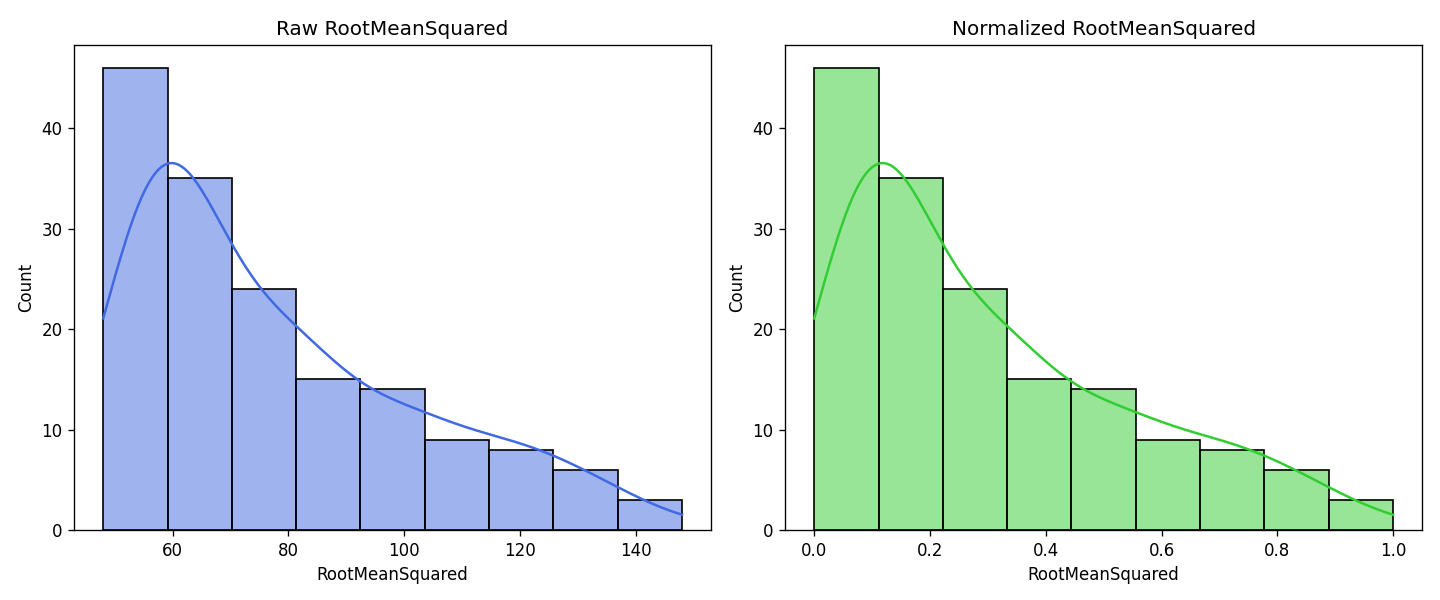
\includegraphics[width=1.1\textwidth]{images/RootMeanSquared.png}
			\caption{Comparisson of feature distribution prior and after the \textit{min-max} normalization.}
			\label{fig1:}
		\end{figure}		



    \section{Evaluation}
		
		\par In the classification stage, two different classifiers have been trained and evaluated, a Random Forest classifier
		and a MultiLayer Perceptron Neural Network. Classification evaluation examined using different configurations of features
		in order to be able to compare the contribution of each of the feature sets in the classification accuracy and estimate
		the degree of their contribution.

		The Random Forest model, an ensemble based method known for its robustness and interpretability, 
		was trained using 100 decision trees and a fixed random seed for ensuring reproducibility. 
		For the second classifier, the neural network model was configured having
		two hidden layers comprising 100 and 50 neurons respectively, trained 
		for up to 500 iterations.

	\subsection{Classification with texture, shape and statistical features}

		Classification evaluation with texture, shape and statistical features results are presented below.
	
		\begin{figure}[h]
			\centering
			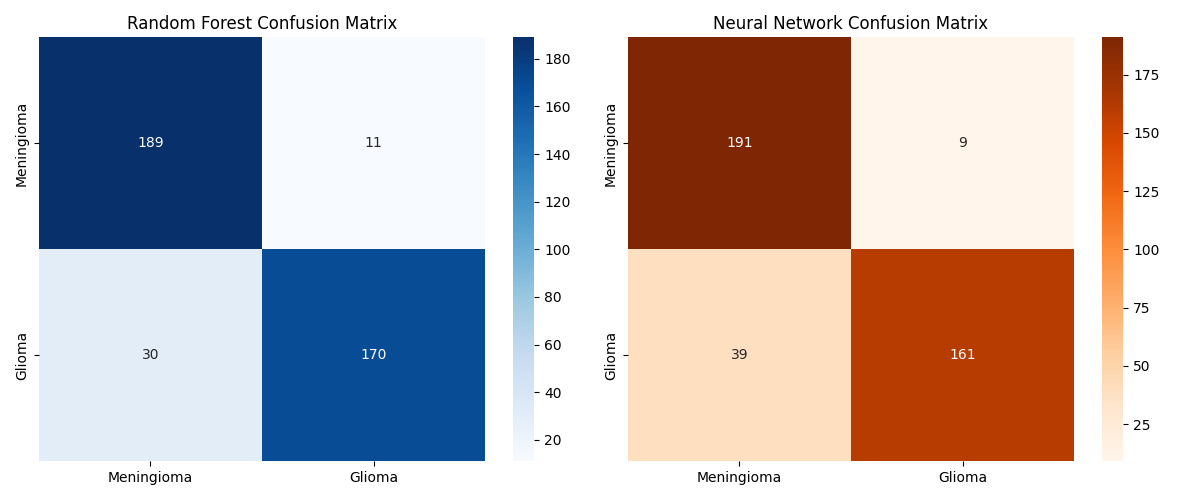
\includegraphics[width=1.1\textwidth]{images/classification_pyradiomics.png}
			\caption{Metric results.}
			\label{fig1:}
		\end{figure}		

		\begin{figure}[h]
			\centering
			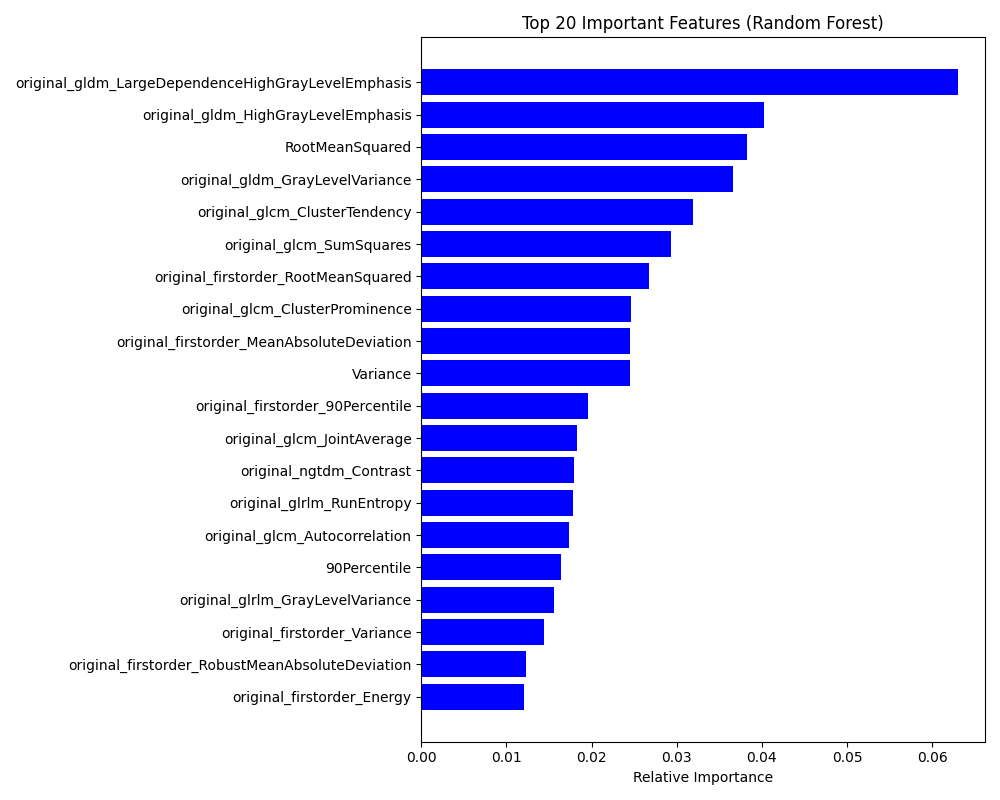
\includegraphics[width=0.7\textwidth]{images/top20_rf_pyradiomics.png}
			\caption{Top20 features of RF.}
			\label{fig1:}
		\end{figure}		

		\begin{figure}[H]
			\centering
			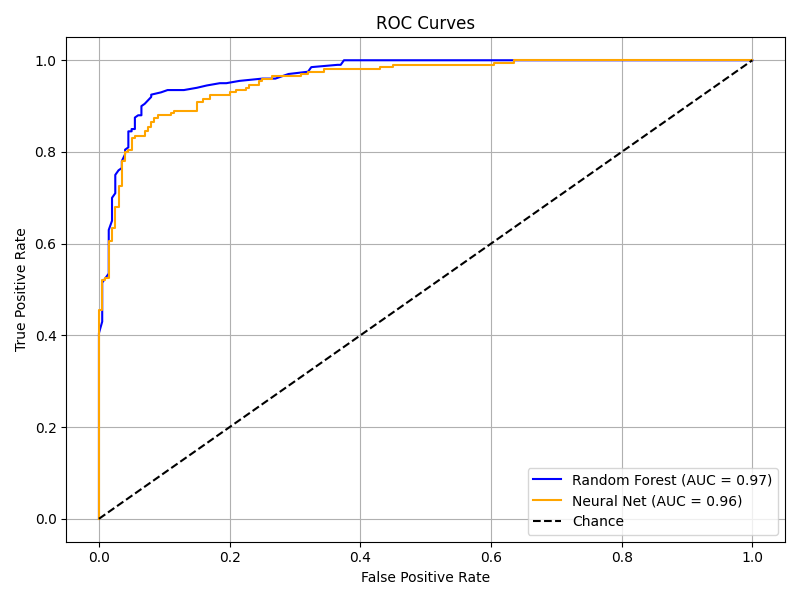
\includegraphics[width=0.9\textwidth]{images/roc_pyradiomics.png}
			\caption{RoC curves for RF and MLP-nn.}
			\label{fig1:}
		\end{figure}		

		\begin{figure}[H]
			\centering
			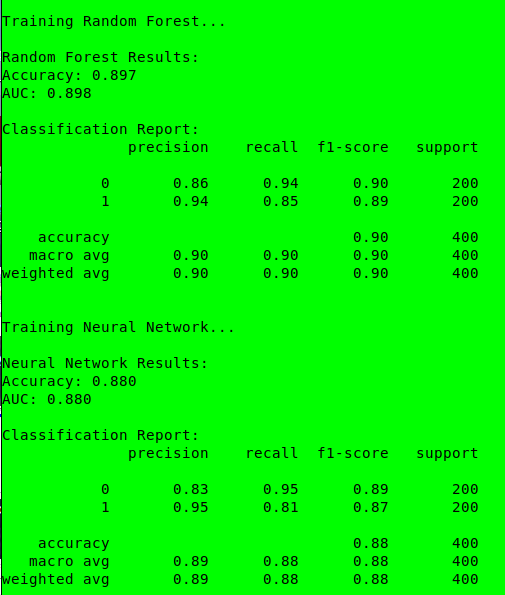
\includegraphics[width=0.5\textwidth]{images/report_pyradiomics.png}
			\caption{Classification report}
			\label{fig1:}
		\end{figure}		

	\subsection{Classification with frequency features}
		

		Classification evaluation's results using the extracted frequency features are presented in the 
		next figures.

		\begin{figure}[h]
			\centering
			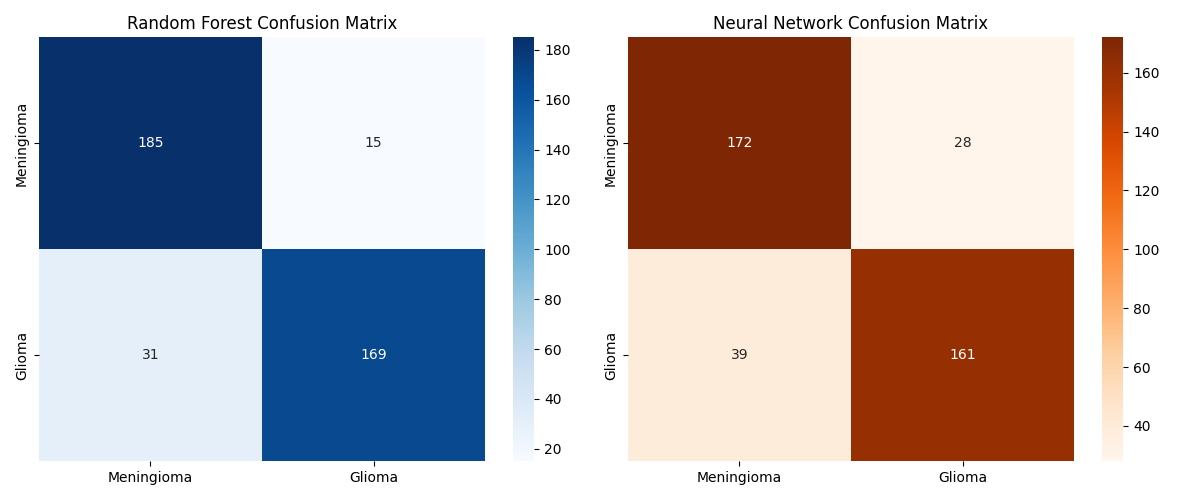
\includegraphics[width=1.1\textwidth]{images/freq_metrics.png}
			\caption{Metric results.}
			\label{fig1:}
		\end{figure}		

		\begin{figure}[h]
			\centering
			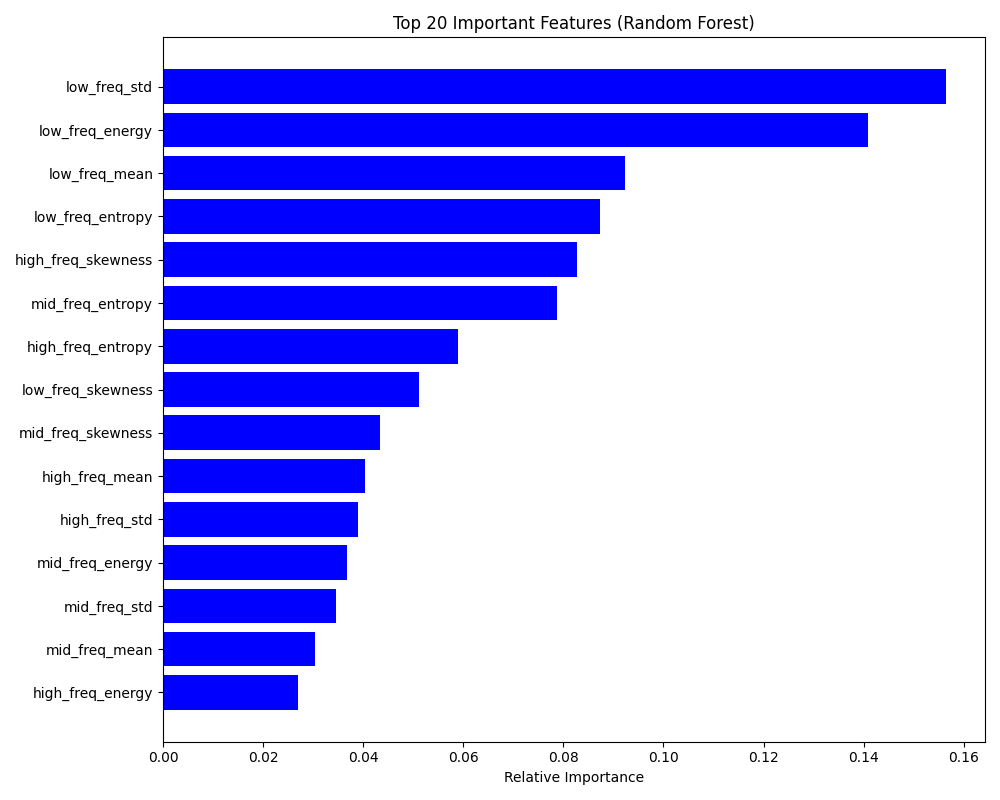
\includegraphics[width=0.7\textwidth]{images/freq_top_rf.png}
			\caption{Top20 features of RF.}
			\label{fig1:}
		\end{figure}		

		\begin{figure}[H]
			\centering
			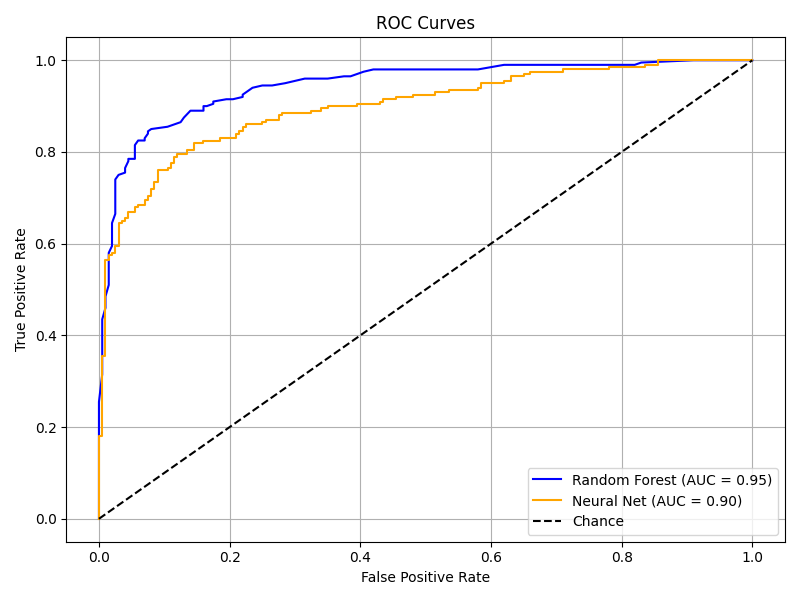
\includegraphics[width=0.9\textwidth]{images/freq_roc.png}
			\caption{RoC curves for RF and MLP-nn.}
			\label{fig1:}
		\end{figure}		

		\begin{figure}[H]
			\centering
			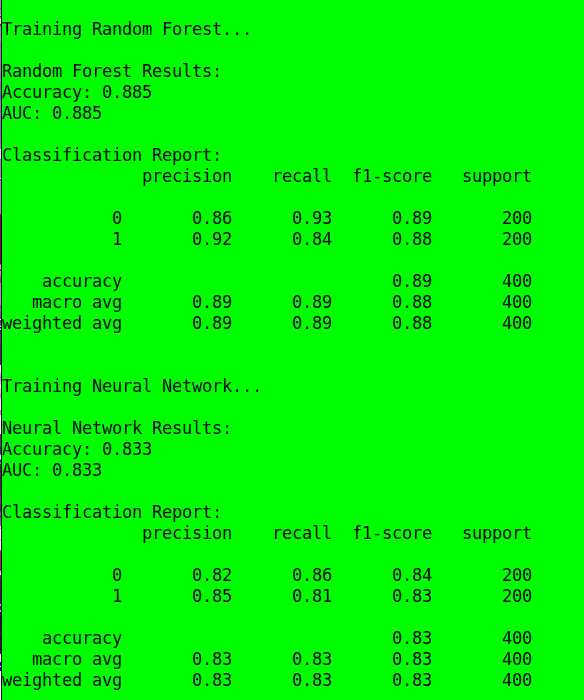
\includegraphics[width=0.5\textwidth]{images/report_freq.png}
			\caption{Classification report}
			\label{fig1:}
		\end{figure}		


	\subsection{Classification utilizing all features}

		Classification results utilizing all the available features extracted are presented in following figures.
		\begin{figure}[H]
			\centering
			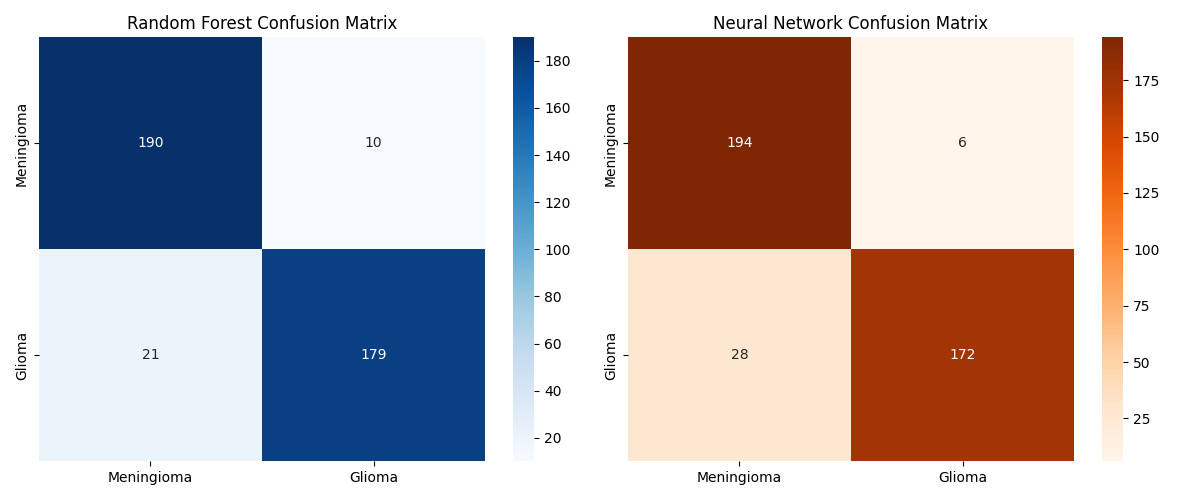
\includegraphics[width=1.1\textwidth]{images/Metrics_all_features.png}
			\caption{Metric results.}
			\label{fig1:}
		\end{figure}		

		\begin{figure}[H]
			\centering
			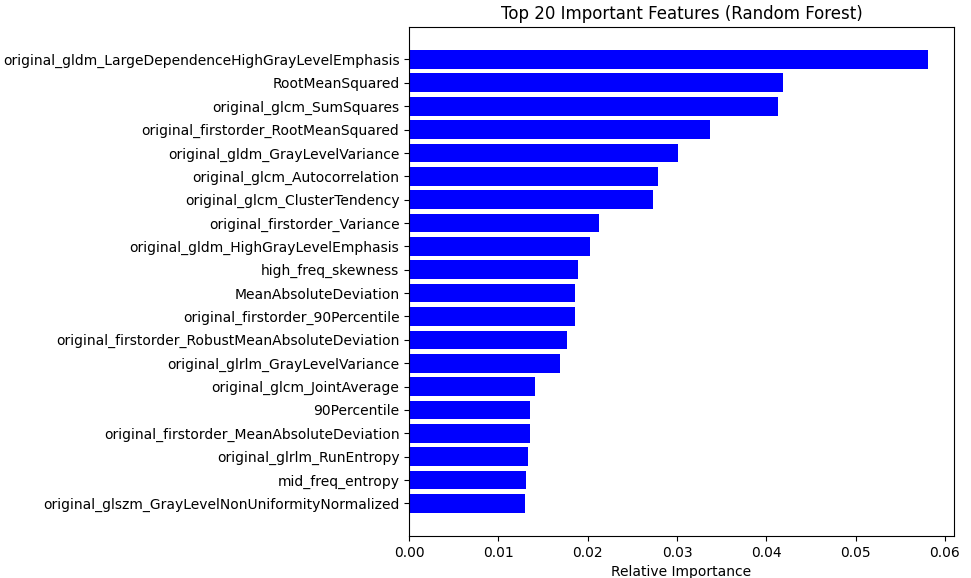
\includegraphics[width=0.7\textwidth]{images/top20features_all_features_rf.png}
			\caption{Top20 features of RF.}
			\label{fig1:}
		\end{figure}		

		\begin{figure}[H]
			\centering
			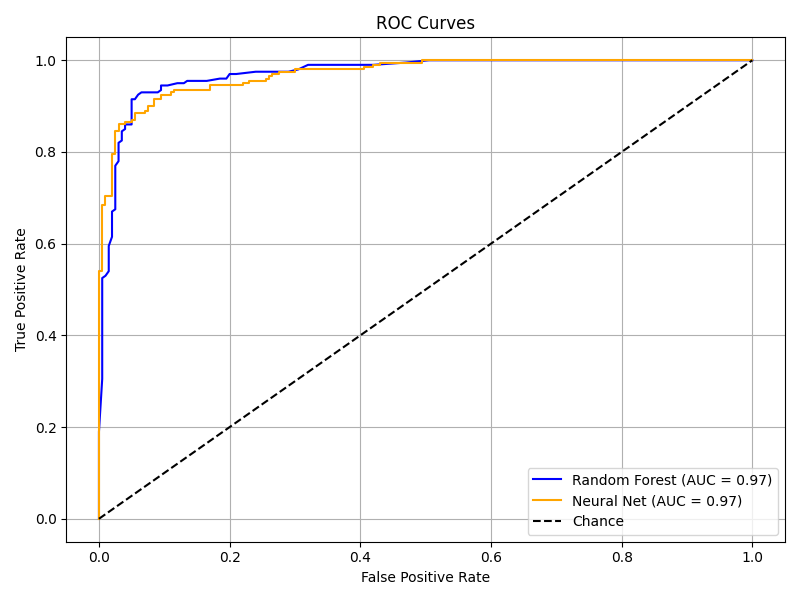
\includegraphics[width=0.9\textwidth]{images/roc_curves_all_features.png}
			\caption{RoC curves for RF and MLP-nn.}
			\label{fig1:}
		\end{figure}		

		\begin{figure}[H]
			\centering
			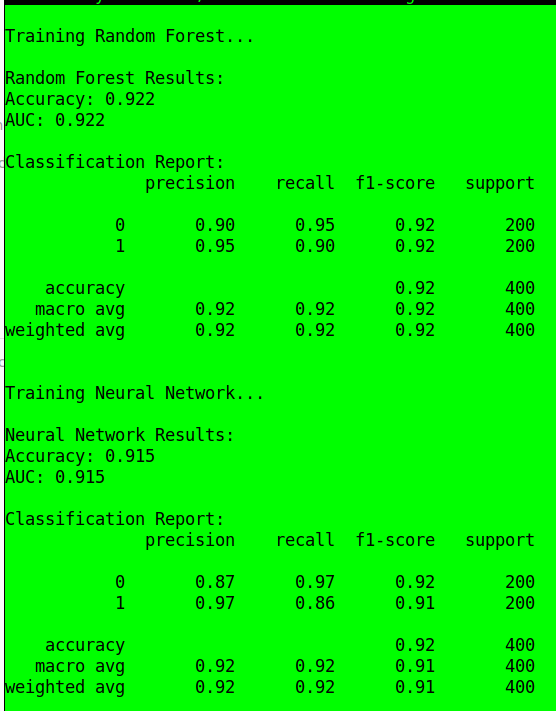
\includegraphics[width=0.5\textwidth]{images/report_all_features.png}
			\caption{Classification report}
			\label{fig1:}
		\end{figure}		


\subsection{Evaluation Findings}

The results from the three feature configurations demonstrate that combining all available 
features (texture/shape/statistical and frequency domain features) yields the highest 
classification performance. Key observations include:

\begin{itemize}
    \item \textbf{Feature set comparison:}

    \begin{itemize}
        \item \textit{All features} achieved the best results, underscoring the complementary nature of radiomic, custom-designed, 
		and frequency-domain features.
        \item \textit{Texture/shape/statistical features} alone provided competitive performance, 
		suggesting and confirming the strong discriminative power they yield for tumor classification.
        \item \textit{Frequency features} were slightly less effective in isolation 
		but contributed meaningfully when integrated with other features.
    \end{itemize}
    
    \item \textbf{Glioma classification improvement:}
	    Misclassification rates for glioma dropped significantly (from 31 out of 200 MRIs (15.5\%) using texture/shape features 
		only to 21 out of 200 MRIs (10.5\%)  and from 38 out of 200 MRIs (19\%) using texture/shape features 
		only to 28 out of 200 MRIs (14\%)  )
		when all features were utilized. This highlights the importance of hybrid feature engineering for capturing tumor heterogeneity.
    
    \item \textbf{Model performance:}
		The Random Forest classifier consistently outperformed the MLP neural network across all configurations, 
		particularly in terms of interpretability (e.g., feature importance rankings) and robustness (AUC metrics).
\end{itemize}




		\subsection{Classifier Optimization}

		At this point, hyperparameter optimization is explored in order to achieve better classification
		results utilizing the created models.
		In our workflow,  first a Random Forest classifier was utilized with hyperparameter tuning 
		to identify the 30 most important features from the dataset. 
		The hyperparameters such as the number of trees (n\_estimators), tree depth (max\_depth), 
		minimum samples per split and leaf (min\_samples\_split, min\_samples\_leaf), 
		and others are optimized using randomized search with cross-validation. 
		
		This ensures that the Random Forest model is tuned for the purpose of capturing
		the most relevant patterns in the data but also for preventing overfitting. 
		After determining the feature importances, the top 30 features are selected as inputs for the next step.
		These selected features are then fed into a neural network (MLPClassifier) 
		with fixed hyperparameters (e.g., activation function, solver, learning rate, and number of iterations) for
		performing the final classification. 
		Using the best subset of features reduces dimensionality and noise, and can improve the 
		neural network’s performance and training efficiency, 
		while benefiting from complementary strengths of both models for robust classification.
		
		Results from tuned-modified models in this way are presented below.


		\begin{figure}[H]
			\centering
			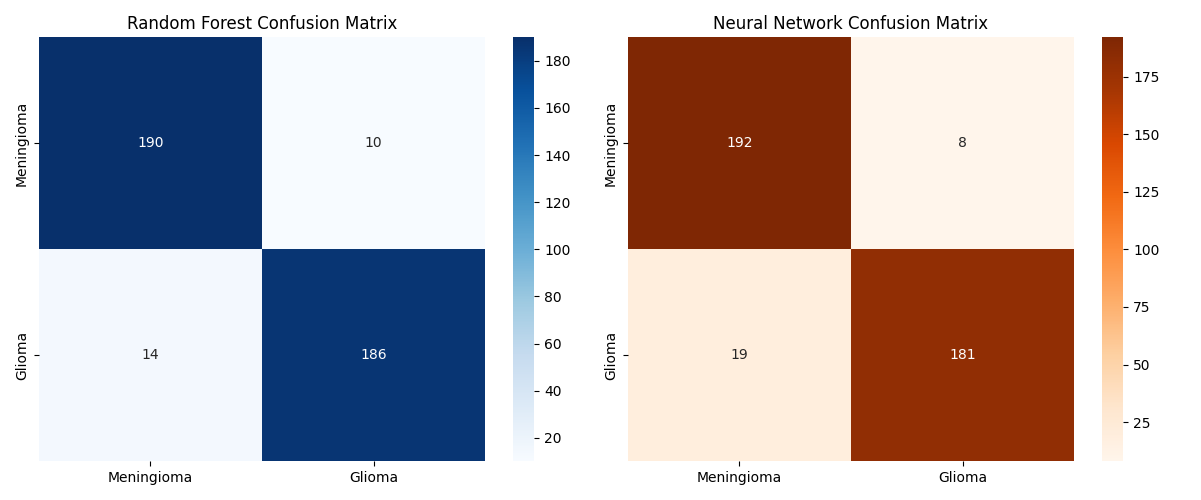
\includegraphics[width=1.1\textwidth]{images/metrics_hyper.png}
			\caption{Metric results.}
			\label{fig1:}
		\end{figure}		

		\begin{figure}[H]
			\centering
			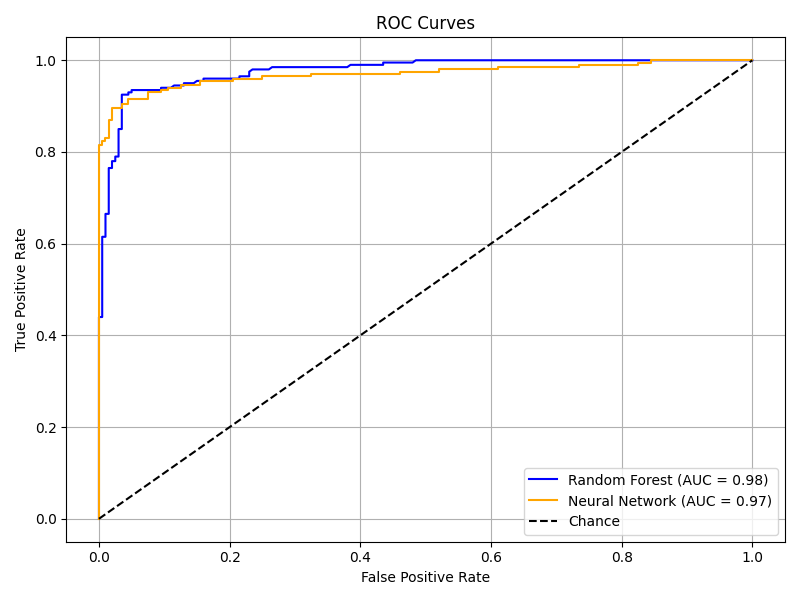
\includegraphics[width=0.9\textwidth]{images/roc_hyper.png}
			\caption{RoC curves for RF and MLP-nn.}
			\label{fig1:}
		\end{figure}		

	
		After hyperparameter tuning, the Random Forest classifier’s accuracy improved from 0.922 to 0.94, 
		indicating a notable gain of approximately 1.8%. 
		This improvement suggests that optimizing 
		parameters like the number of trees, tree depth, and feature selection/reduction helped the model to
		better capture patterns in the data, resulting in more accurate predictions.

		In a similar way, the neural network 's accuracy increased from 0.915 to 0.932, 
		a gain of about 1.7\%. 
		This demonstrates that tuning hyperparameters such as the network architecture, 
		learning rate, and using only the top 30 features selected by Random Forest's model
		allowed  better generalization on the test data.

		In overall, both models benefited from hyperparameter optimization, 
		with the Random Forest showing a slightly higher accuracy gain. 
		Improvements like these highlight the importance of fine tuning model settings 
		in order to achieve maximization in classification performance, 
		even in cases of starting from already strong baseline models.
		

		As for the model agreement, a comparative analysis plot in Figure X, 
		shows that both classifiers largely agree and perform well together, 
		with most samples correctly identified by both.
		Each model also has some unique correct predictions, 
		demonstrating by this their complementary strengths.
		More strategies could be employed (f.e voting etc) that could improve an overall
		system's performance.
		There is a relatively small number of samples misclassified by both models(11/400) samples,
		highlighting area for further improvements for this project.
		
		\begin{figure}[H]
			\centering
			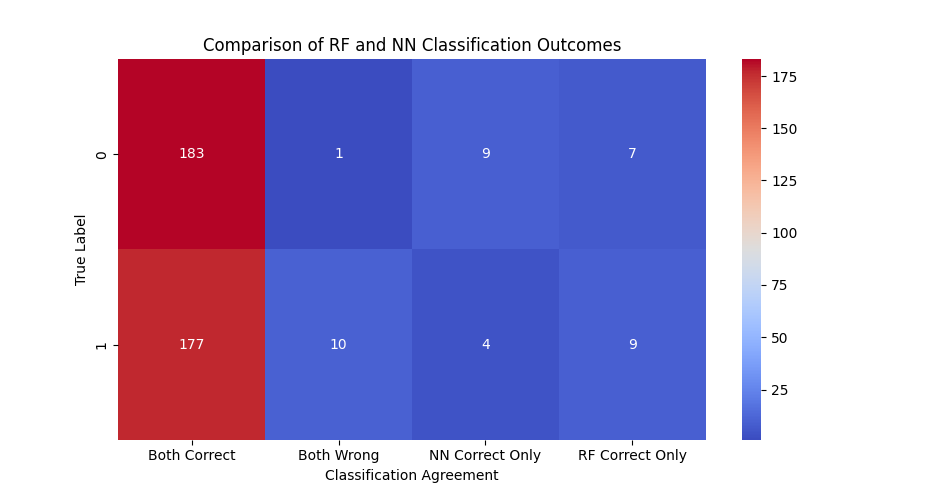
\includegraphics[width=0.9\textwidth]{images/comparison.png}
			\caption{RoC curves for RF and MLP-nn.}
			\label{fig1:}
		\end{figure}		


\section{Histogram Matching enchancement}


Analysis of the histograms of the MRI images on the dataset is performed
and is presented below. Results of analysing the intensitis of the 
MRI images per category (Figure 5.1)
demonstrate that unnormalized intensity distributions introduce scanner 
or acquisition protocol-dependent variability that
could dominate the signal of interest. 
Via the application of histogram matching technique image 
intensities should be aligned on the intensity distributions 
while preserving the relative contrast relationships 
essential for the exact tumor classification.

		\begin{figure}[H]
			\centering
			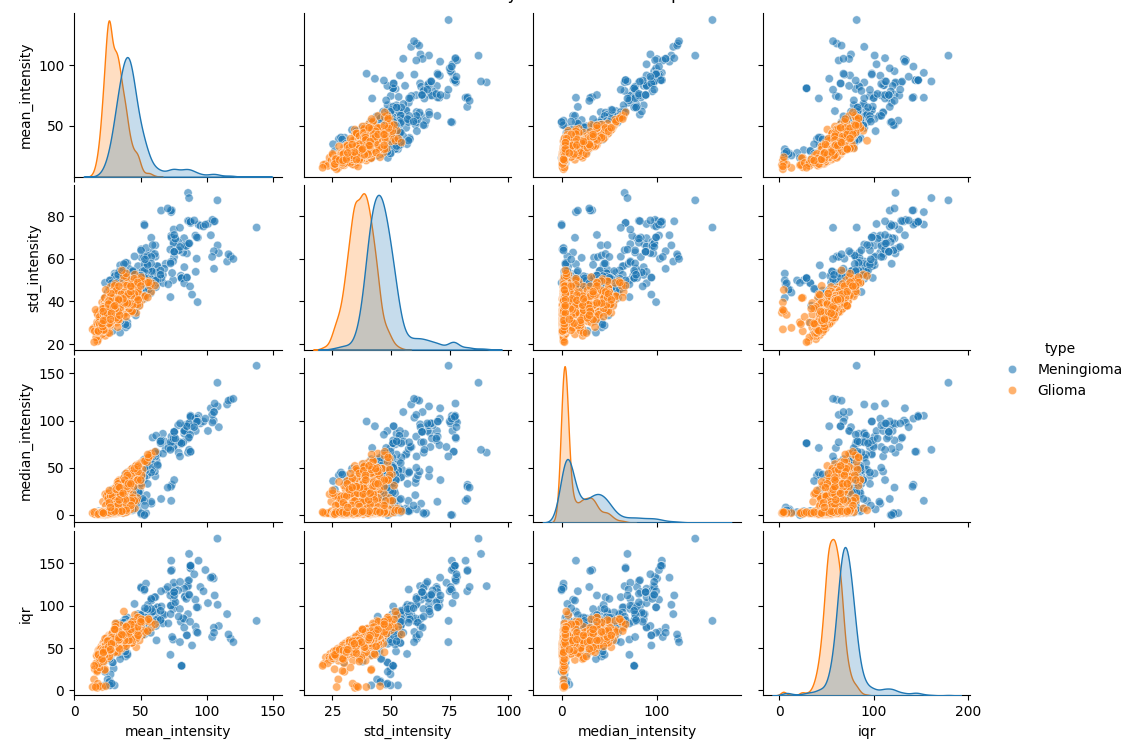
\includegraphics[width=1.0\textwidth]{images/histogram_analysis_unmatched.png}
			\caption{Analysis plot of all the MRI histograms.}
			\label{fig1:}
		\end{figure}		


Also in Figure 5.2 we can observe graphical the distribution intensities of the MRIs for both classes.
		\begin{figure}[H]
			\centering
			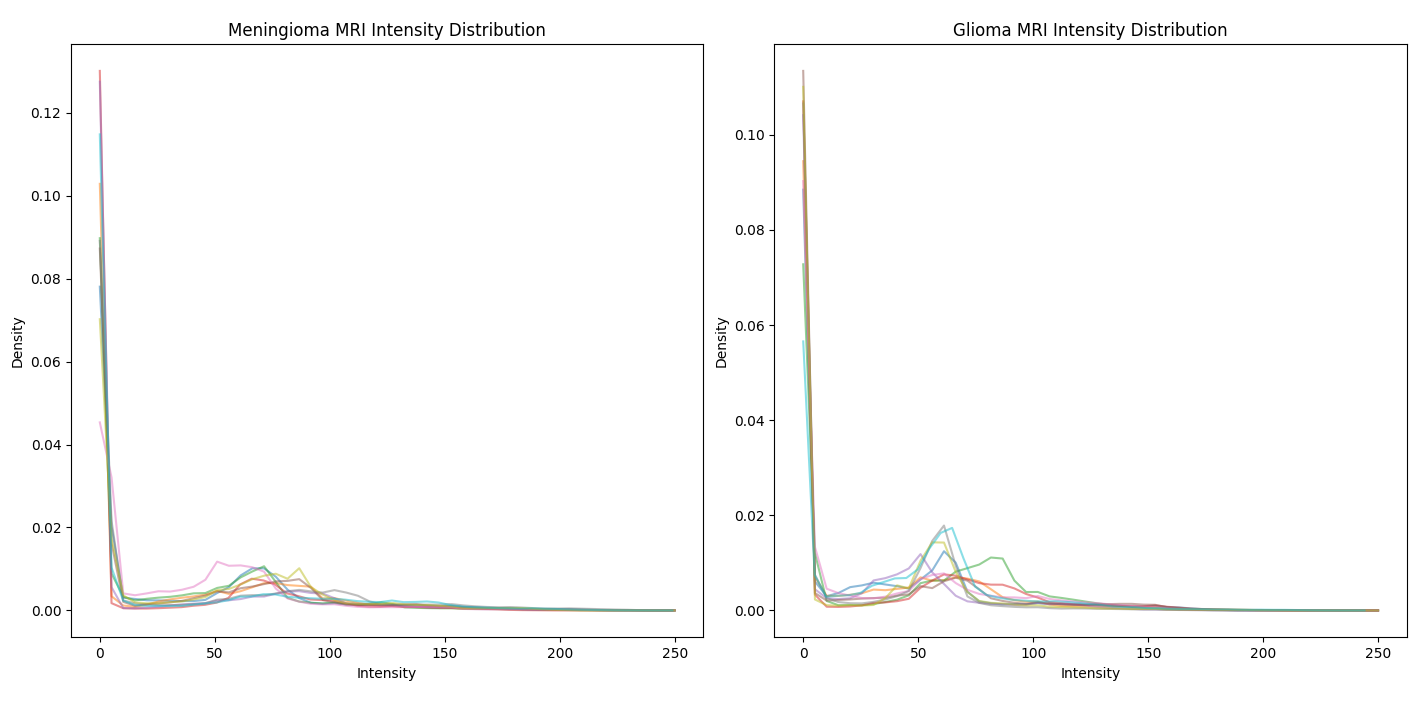
\includegraphics[width=1.0\textwidth]{images/Unmatched_intensity_distributions.png}
			\caption{Intensity distributions of MRI histograms.}
			\label{fig1:}
		\end{figure}		




\subsection{Reference image selection}

For the proccess of the selection of an optimal reference image for histogram matching, MRI images have been systematically evaluated
from the dataset (sampling 300 candidates by default) and choose the one that maximized class separability after histogram matching.
Each candidate reference image, is tested on a subset of images (20 per class) 
by performing histogram matching and then calculating a separability score based on the 
difference in mean intensities between glioma and meningioma classes 
normalized by their combined standard deviation. The candidate that produces the highest score (indicating by that
the best separation between classes after histogram matching) is selected as the final reference image. 
By following such an approach chooses a reference that maintains discriminative 
intensity characteristics between the two tumor types while using a single unbiased 
reference for all images.

The effect of histogram matching on 500 sampled MRIs belonging to meningioma category and 500 sampled MRIs belonging to glioma category is 
visualized in Figure 16.

		\begin{figure}[H]
			\centering
			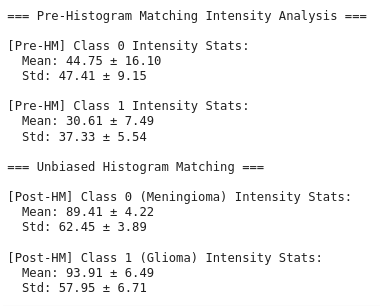
\includegraphics[width=0.8\textwidth]{images/pre_hm_stats.png}
			\caption{Intensity metrics of 1000 MRIs prior histogram matching.}
			\label{fig1:}
		\end{figure}		

Prior to histogram matching, there was a greater difference in intensity statistics(mean and standard deviation)
between the two classes. 
Meningioma MRIs exhibited a higher mean intensity (44.75 ± 16.10) and 
standard deviation (47.41 ± 9.15) compared to glioma MRIs (30.61 ± 7.49 mean; 37.33 ± 5.54 std), 
indicating class-specific variations in brightness and contrast. 
After performing histogram matching, the intensity distributions of both classes are aligned more closely 
to a common reference, resulting in similar mean intensities (89.41 ± 4.22 for healthy, 93.91 ± 6.49 for tumor) 
and reduced variation in standard deviation between the classes (62.45 ± 3.89 vs. 57.95 ± 6.71). 
This transformation effectively normalized intensity-related differences, allowing downstream radiomic feature 
extraction and classification models to focus more on structural and textural patterns.


\subsection{Evaluation of classification with histogram matching}

		Utilizing the histogram matching with the previously described reference image selection method,
		and by extracting all the features, classification has been re-evaluated.
		Results of using all the available features extracted from histogram matched MRIs 
		are presented in following figures.
		\begin{figure}[H]
			\centering
			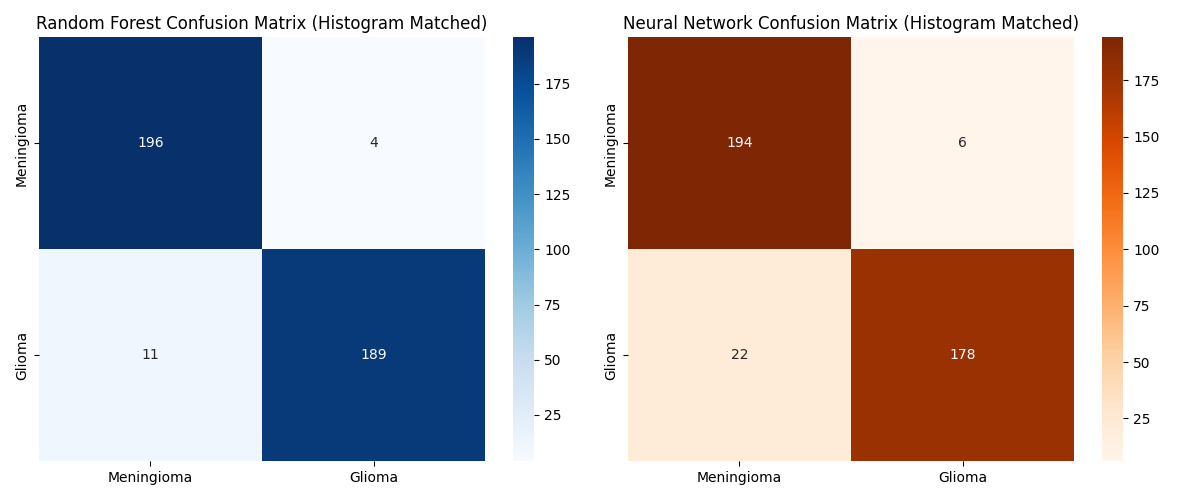
\includegraphics[width=1.1\textwidth]{images/metrics_hm.png}
			\caption{Metric results.}
			\label{fig1:}
		\end{figure}		

		\begin{figure}[H]
			\centering
			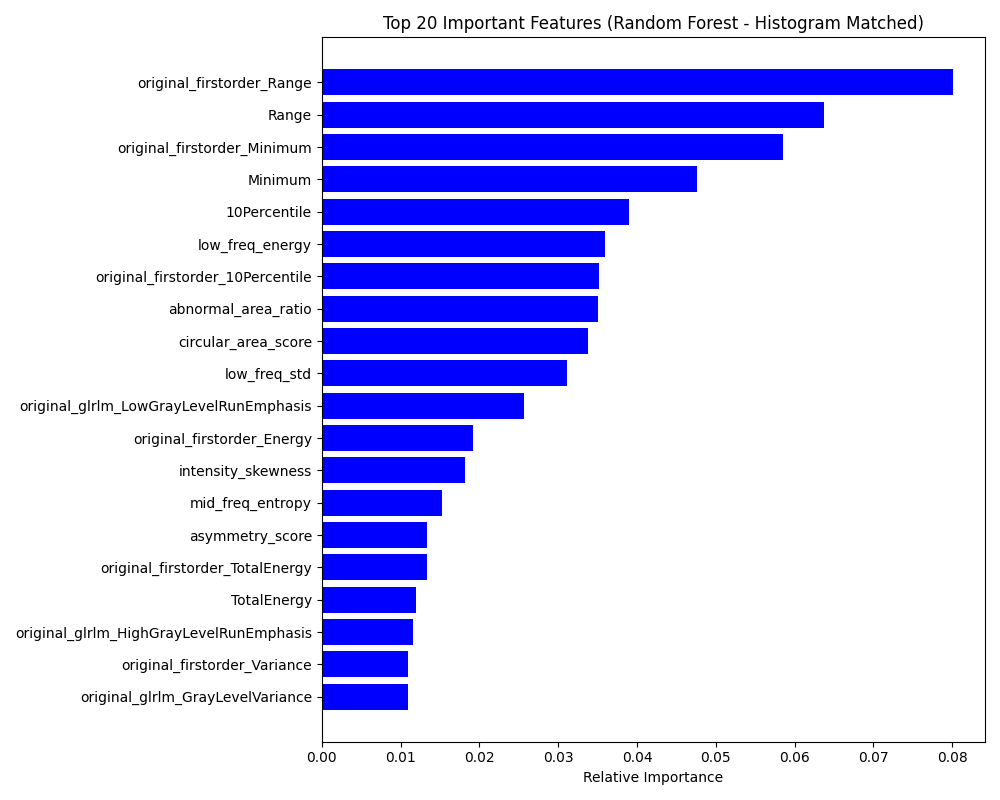
\includegraphics[width=0.7\textwidth]{images/top20_rf_hm.png}
			\caption{Top20 features of RF.}
			\label{fig1:}
		\end{figure}		

		\begin{figure}[H]
			\centering
			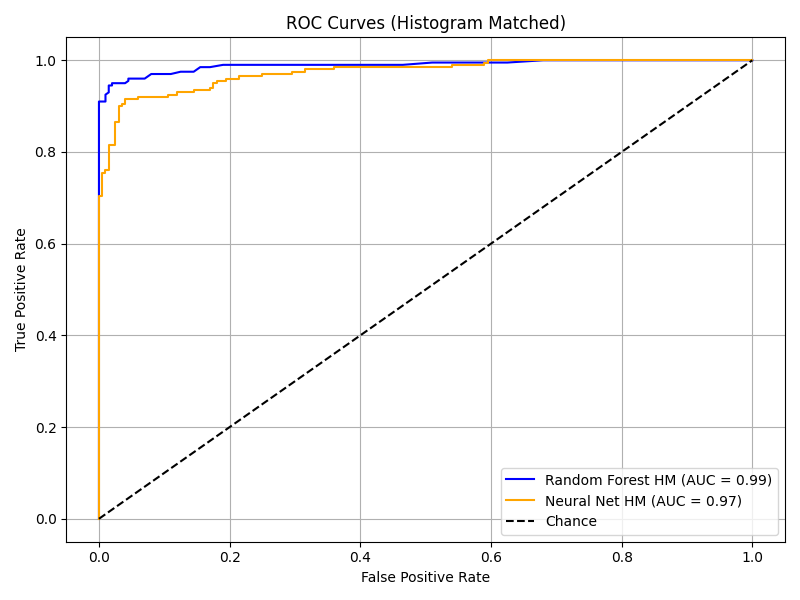
\includegraphics[width=0.9\textwidth]{images/roc_hm.png}
			\caption{RoC curves for RF and MLP-nn.}
			\label{fig1:}
		\end{figure}		

		\begin{figure}[H]
			\centering
			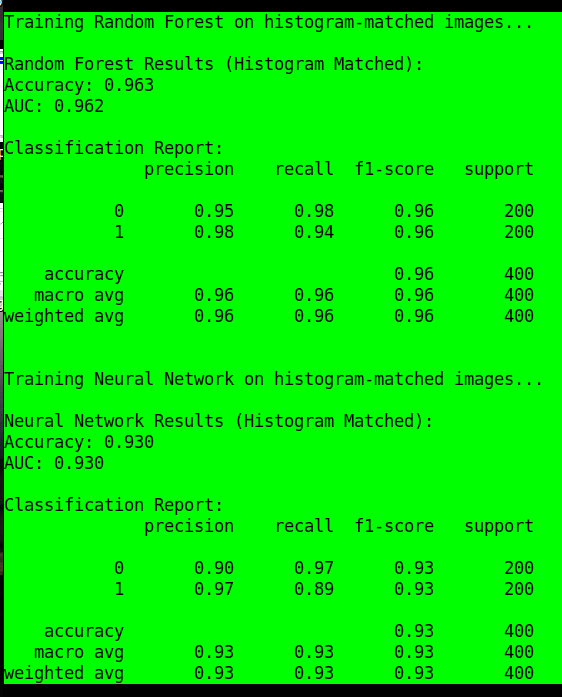
\includegraphics[width=0.5\textwidth]{images/report_hm.png}
			\caption{Classification report}
			\label{fig1:}
		\end{figure}		

Histogram matching with an optimized reference image improved 
classification accuracy by 4.2\% (RF) and 1.5\% (MLP-nn), 
suggesting that the intensity normalization enhances model generalizability. 
The larger gain was observed in the Random Forest and by observing the figure refering to the
top 20 features contribution for the RF-classification we can inspect that four (20\%) of the 
custom extracted features are included in the list.

\section{Conclusion}


\bibliographystyle{plain}

\bibliography{references}
 
\end{document}
